

\documentclass[twocolumn]{article}
\usepackage{pgfplots}

\begin{document}
\begin{figure}
\centering
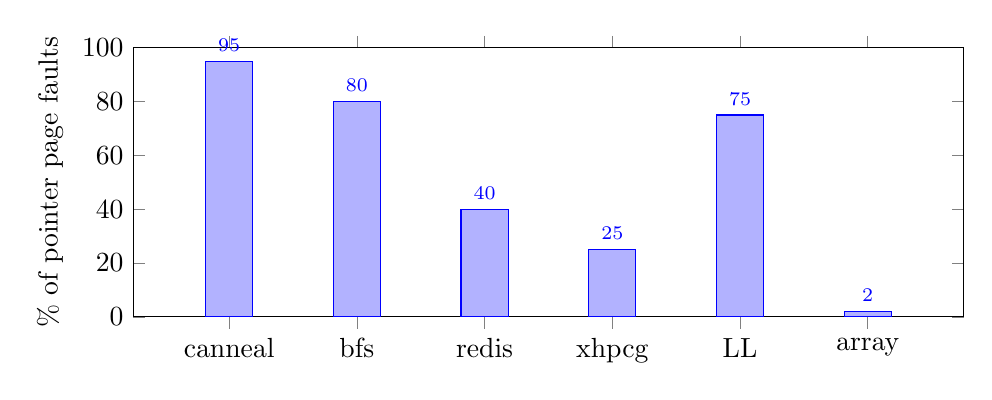
\begin{tikzpicture}
\begin{axis}[
    ybar,
    symbolic x coords={canneal, bfs, redis, xhpcg, LL, array},
    xtick=data,
    xtick distance=1.5, % Adjust the spacing between x-axis markers
    ylabel={\% of pointer page faults},
    width=\columnwidth,
    height=5cm,
    bar width=0.6cm,
    enlarge x limits=0.15,
    ymin=0,
    ymax=100,
    nodes near coords,
    nodes near coords align={vertical},
    every node near coord/.append style={
        font=\scriptsize,
        /pgf/number format/fixed,
        /pgf/number format/precision=2
    },
]
\addplot coordinates {(canneal, 95) (bfs, 80) (redis, 40) (xhpcg, 25) (LL, 75) (array, 2)};
\end{axis}
\end{tikzpicture}
\caption{Pointer page faults for different workloads}
\end{figure}


\begin{figure}
\centering
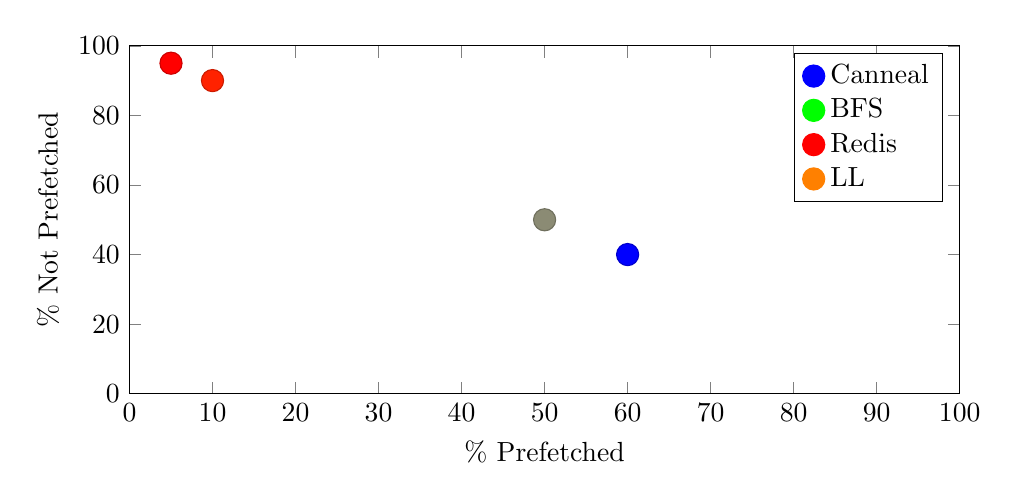
\begin{tikzpicture}
\begin{axis}[
    scatter,
    only marks,
    width=\columnwidth,
    height=6cm,
    xlabel={\% Prefetched},
    ylabel={\% Not Prefetched},
    xmin=0,
    xmax=100,
    ymin=0,
    ymax=100,
    at={(0.75,0.25)}, % Adjust position of the axis
    anchor=north east,
    legend style={
        at={(0.98,0.98)},
        anchor=north east,
        cells={anchor=west},
        legend cell align=left,
        fill=white, % Background color of the legend
        draw=black, % Border color of the legend
    },
]
\addplot[mark size=4, color=blue] coordinates {(5, 95)};
\addlegendentry{Canneal}
\addplot[mark size=4, color=green] coordinates {(60, 40)};
\addlegendentry{BFS}
\addplot[mark size=4, color=red] coordinates {(10, 90)};
\addlegendentry{Redis}
\addplot[mark size=4, color=orange] coordinates {(50, 50)};
\addlegendentry{LL}
\end{axis}
\end{tikzpicture}
\caption{Scatter plot showing \% Prefetched vs. \% Not Prefetched for different workloads.}
\end{figure}



\begin{figure}
\centering
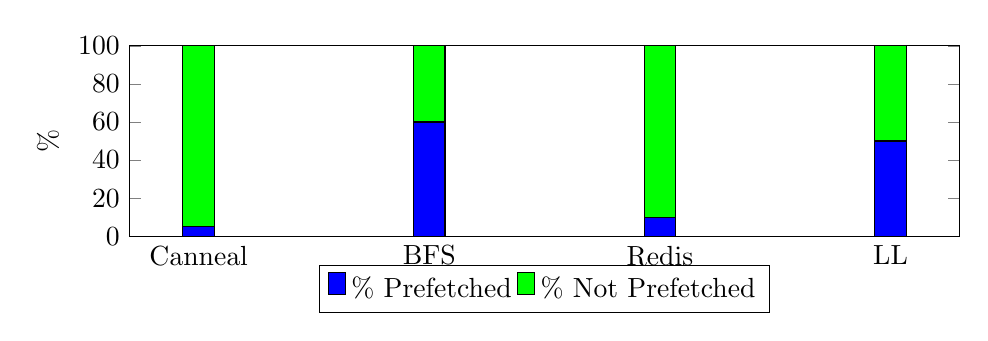
\begin{tikzpicture}
\begin{axis}[
    ybar stacked,
    bar width=0.4cm,
    width=\columnwidth,
    height=4cm,
    xlabel={Workloads},
    ylabel={\%},
    symbolic x coords={Canneal, BFS, Redis, LL},
    xtick=data,
    ymin=0,
    ymax=100,
    legend style={
        at={(0.5,-0.15)},
        anchor=north,
        legend columns=-1, % Automatically arrange legend entries
    },
]
\addplot[fill=blue] coordinates {(Canneal, 5) (BFS, 60) (Redis, 10) (LL, 50)};
\addplot[fill=green] coordinates {(Canneal, 95) (BFS, 40) (Redis, 90) (LL, 50)};
\legend{\% Prefetched, \% Not Prefetched}
\end{axis}
\end{tikzpicture}
\caption{Stacked bar chart showing \% Prefetched and \% Not Prefetched for different workloads.}
\end{figure}





\begin{table*}
\centering
\begin{tabularx}{\textwidth}
\hline
\textbf{Column 1} & \textbf{Column 2} & \textbf{Column 3} & \textbf{Column 4} \\
\hline
Data 1 & Data 2 & Data 3 & Data 4 \\
Data 5 & Data 6 & Data 7 & Data 8 \\
\hline
\end{tabularx}
\caption{A full-width table that spans the page.}
\end{table*}


\end{document}